\section{What these benchmarks can resolve}
\label{sec:resolution}

Throughout we take the acquisitions needed to detect an effect $d$ at 80\% power
and two-sided $\alpha = 0.05$ as $n = (2.80\,s/d)^2$, with $s$ the paired per-fold
standard deviation, $2.80 = z_{0.975} + z_{0.80}$. Each of our effects carries its
measured paired spread. The normal approximation understates the paired $t$-test
requirement by two to three at these sample sizes, so the values are planning
approximations rather than exact thresholds.

\begin{figure}[tb]
\centering
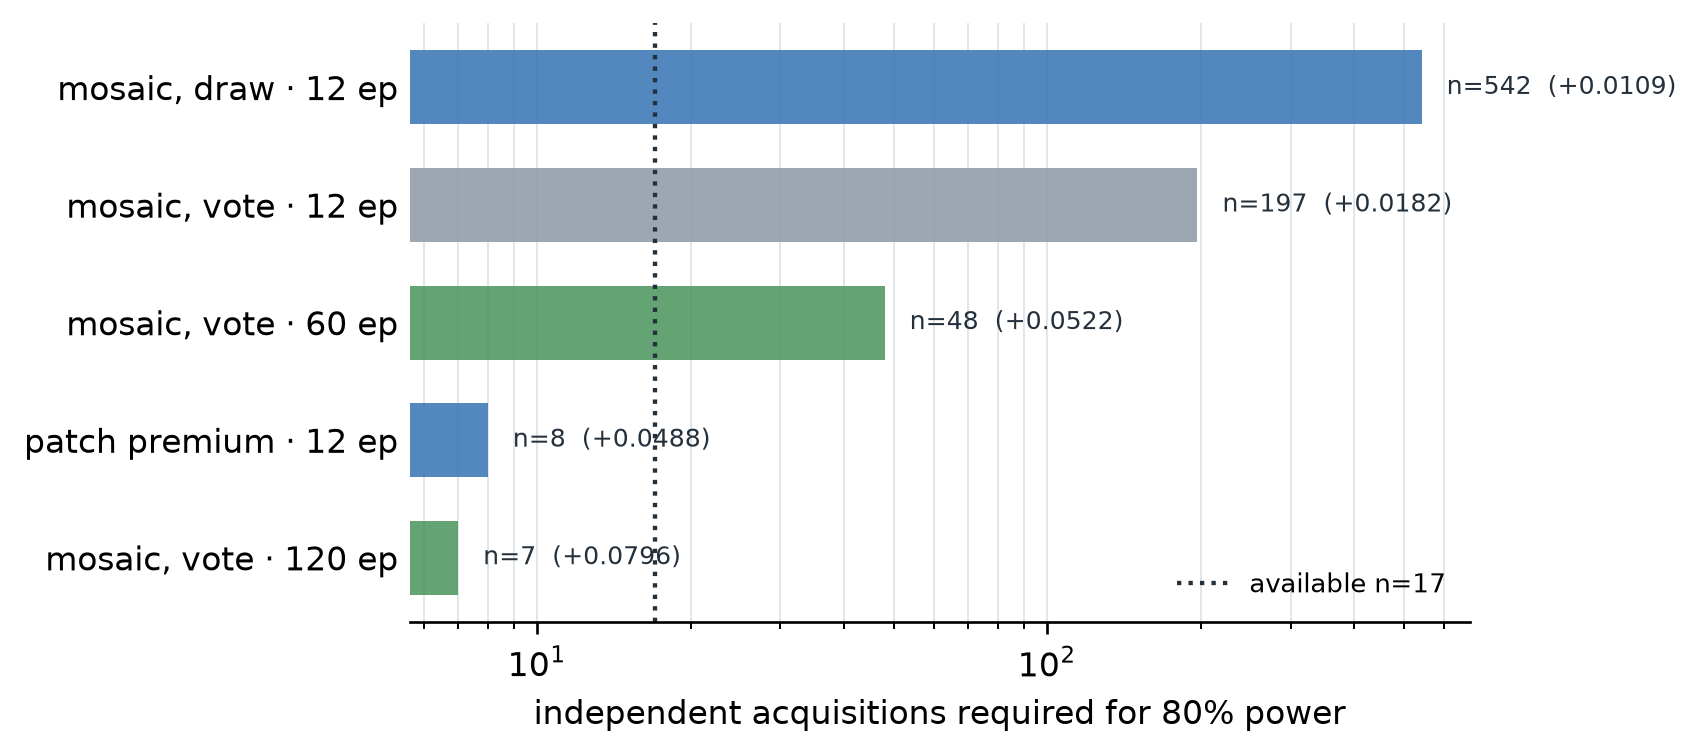
\includegraphics[width=\linewidth]{figures/required_sample_size.png}
\caption{Acquisitions required to detect our artefact-premium estimates at 80\%
power, log axis. The vertical line marks the 17 available acquisitions. Green bars
are longer-budget sensitivity results supported by summary logs rather than
per-run JSON and checkpoints.}
\label{fig:power}
\end{figure}

We define the \emph{artefact premium} as a difference in differences: the mIoU gap
between a U-Net and a context-free threshold baseline on the closed-loop labels,
minus the same gap on the repaired labels, with both arms scored on identical
pixels. It is the share of the network's apparent advantage that survives only
because of how the labeller was implemented. The same power calculation applies to
it.

\begin{table}[tb]
\centering
\small
\setlength{\tabcolsep}{4pt}
\begin{tabular}{lcccc}
\toprule
 & premium & sd & $t$ & required $n$ \\
\midrule
\multicolumn{5}{l}{\emph{scoring convention, at the 12-epoch budget}} \\
patch pixels & $+0.0488$ & $0.0489$ & $4.12$ & 8 \\
mosaic, vote & $+0.0182$ & $0.0910$ & $0.82$ & 197 \\
mosaic, draw & $+0.0109$ & $0.0903$ & $0.50$ & 542 \\
\midrule
\multicolumn{5}{l}{\emph{training budget, under mosaic-vote scoring}} \\
12 epochs & $+0.0182$ & $0.0910$ & $0.82$ & 197 \\
60 epochs & $+0.0522$ & $0.1290$ & $1.67$ & 48 \\
120 epochs & $\mathbf{+0.0796}$ & $\mathbf{0.0747}$ & $\mathbf{4.39}$ & $\mathbf{7}$ \\
\bottomrule
\end{tabular}
\caption{The artefact premium under three scoring conventions and, below, at three
training budgets on the same 17 folds, with the sample size each would need at 80\%
power. Budget aggregates come from the committed run log; per-run JSON and
checkpoints for the 120-epoch arm are not in the release.}
\label{tab:premium}
\end{table}

Patch-pixel scoring needs 8 acquisitions and therefore resolves, but mosaic scoring,
which counts each source pixel once, needs 197 and does not. Applying that convention
to our own result shrinks the premium $2.7\times$ and removes significance. The draw
convention is still more conservative. Estimating rather than fixing the threshold
coefficient gives $\hat\beta=0.711$ (se $0.175$); under it, the patch-scored premium
falls to $t=1.81$.

\paragraph{Training budget.} The committed log reports that the mosaic premium rises
from $+0.0182$ to $+0.0796$ between 12 and 120 epochs, with the change positive in all
17 folds ($t=3.98$); required $n$ falls from 197 to 7. The runner records a
pre-result stopping criterion: 21 of 34 runs reached the 60-epoch cap without early
stopping, compared with 2 of 34 at 120. The 120-epoch result survives every
leave-one-out analysis (minimum $t=4.02$) and four missing-class conventions. These
are useful sensitivity checks, but they remain log-level evidence because the
release lacks their per-run JSON and checkpoints. We therefore do not use them in
the abstract or conclusion.

\paragraph{Multiplicity.} This paper reports many tests, and the results it rests on
are not close to the boundary. Crop alignment at $t = 12.88$ and the dose-response at
$t = 29.84$ would not change interpretation under a Bonferroni factor of 100. The cost
at $t = -4.27$ is $p = 0.0016$ on 10 degrees of freedom, so it tolerates a factor of
about 30 and not 100, which we state because it is the weakest of the three. One
secondary result sits where multiplicity matters and should be read as suggestive: the
transfer collapse sign test at $p = 0.065$. We apply no blanket correction, because a
structural null and an estimated contrast are not the same kind of object.
